\section{Data}

%------------------------------------------------

\subsection{Generation}

\begin{frame}
    \frametitle{Data Generation}

    % Top Block: Common Parameters
    \begin{block}{Simulation Parameters}
        \begin{itemize}
            \item \textbf{Time:} $10\,\text{s}$ duration with $\Delta t = 0.01\,\text{s}$ step.
            \item \textbf{Initialization:} $q_0 \sim \mathcal{U}[-\pi, \pi]$ and $\dot{q}_0 = 0$.
            \item \textbf{System:} Masses ($m_i$) and lengths ($l_i$) are fixed arbitrarily.
        \end{itemize}
    \end{block}

    \vspace{1em}

    % Bottom Section: The 3 Datasets
    \textbf{Generated Datasets}
    \vspace{0.5em}

    \begin{columns}[T]
        \begin{column}{0.33\textwidth}
            \centering
            \color{blue} High Friction \\
            \vspace{0.2em}
            $b = 1.0$
        \end{column}
        
        \begin{column}{0.33\textwidth}
            \centering
            \color{orange} Low Friction \\
            \vspace{0.2em}
            $b = 0.3$
        \end{column}
        
        \begin{column}{0.33\textwidth}
            \centering
            \color{red} No Friction \\
            \vspace{0.2em}
            $b = 0.0$
        \end{column}
    \end{columns}

\end{frame}

%------------------------------------------------

\subsection{Inspection}

\begin{frame}
    \frametitle{Inspecting Generated Datasets}
    
    % --- UPPER ROW ---
    \begin{columns}[T] 
        
        % Up Left
        \begin{column}{0.48\textwidth}
            \centering
            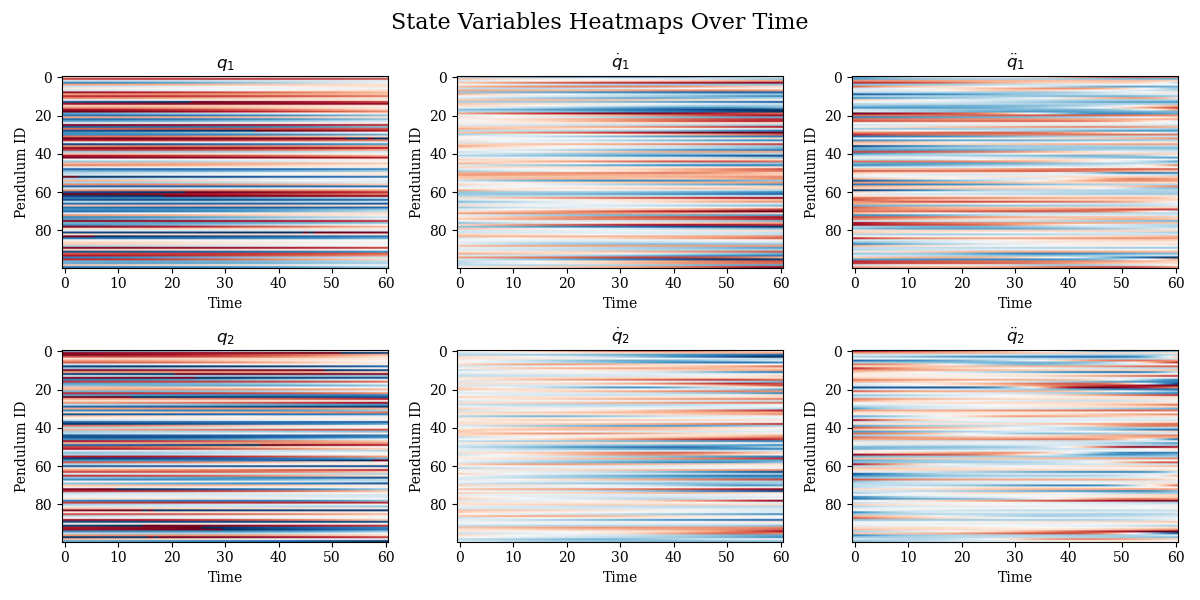
\includegraphics[width=\linewidth]{double_pendulum_highfrict_heatmap.png}
            \vspace{0.2em}
            \scriptsize \textcolor{blue}{High Friction}
        \end{column}
        
        % Up Right
        \begin{column}{0.48\textwidth}
            \centering
            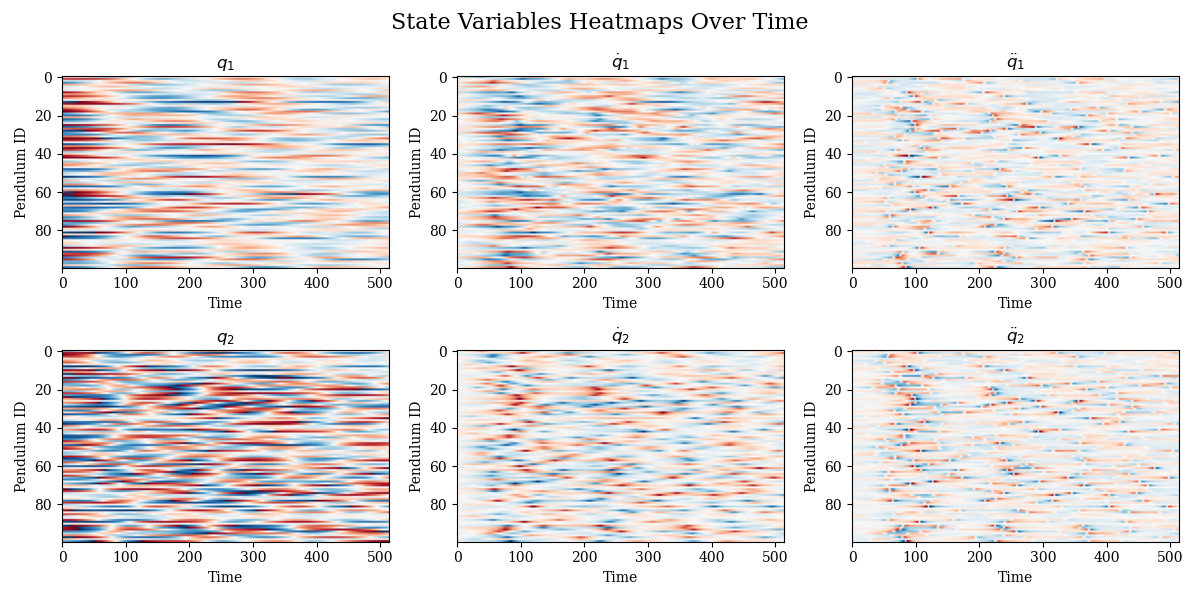
\includegraphics[width=\linewidth]{double_pendulum_lowfrict_heatmap.png}
            \vspace{0.2em}
            \scriptsize \textcolor{orange}{Low Friction}
        \end{column}
        
    \end{columns}

    \vspace{0.5cm} 

    % --- LOWER ROW ---
    \centering
    \begin{minipage}{0.48\textwidth} 
        \centering
        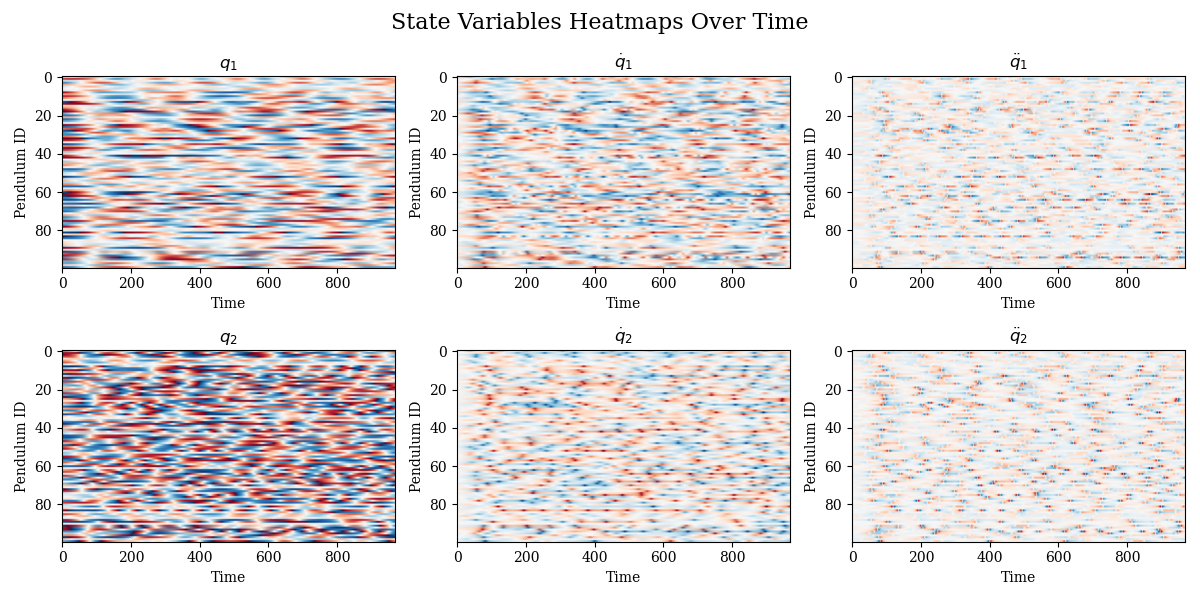
\includegraphics[width=\linewidth]{double_pendulum_nofrict_heatmap.png}
        \vspace{0.2em}
        \scriptsize \textcolor{red}{No Friction}
    \end{minipage}

\end{frame}

\begin{frame}
    \frametitle{Inspecting Generated Datasets}
    
    % --- UPPER ROW ---
    \begin{columns}[T] 
        
        % Up Left
        \begin{column}{0.48\textwidth}
            \centering
            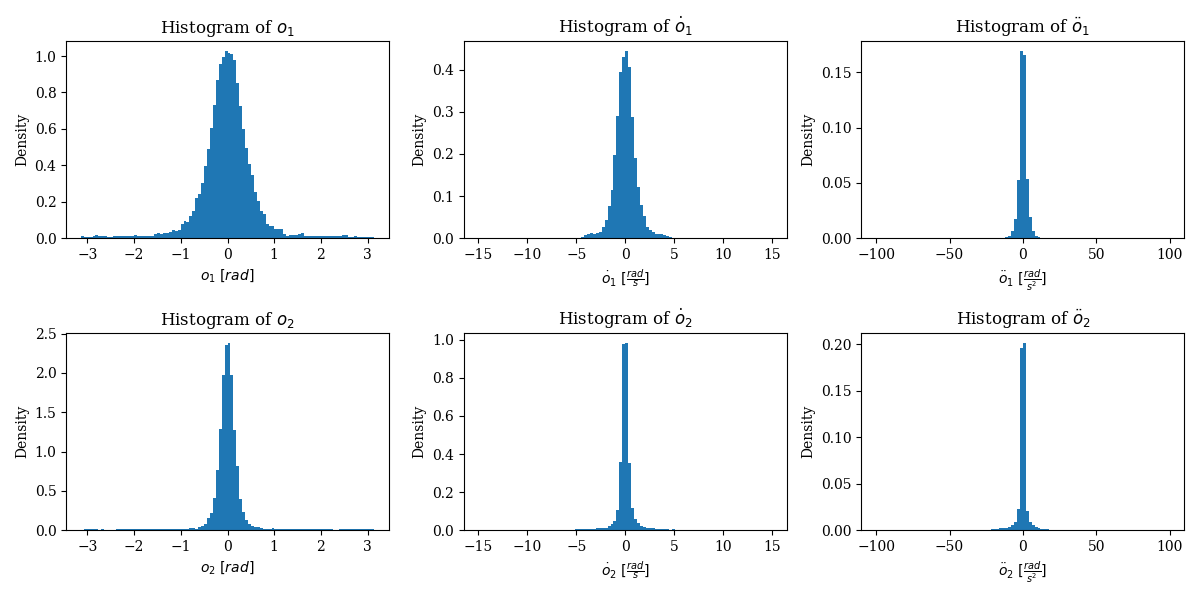
\includegraphics[width=\linewidth]{histogram_pendulum_highfrict.png}
            \vspace{0.2em}
            \scriptsize \textcolor{blue}{High Friction}
        \end{column}
        
        % Up Right
        \begin{column}{0.48\textwidth}
            \centering
            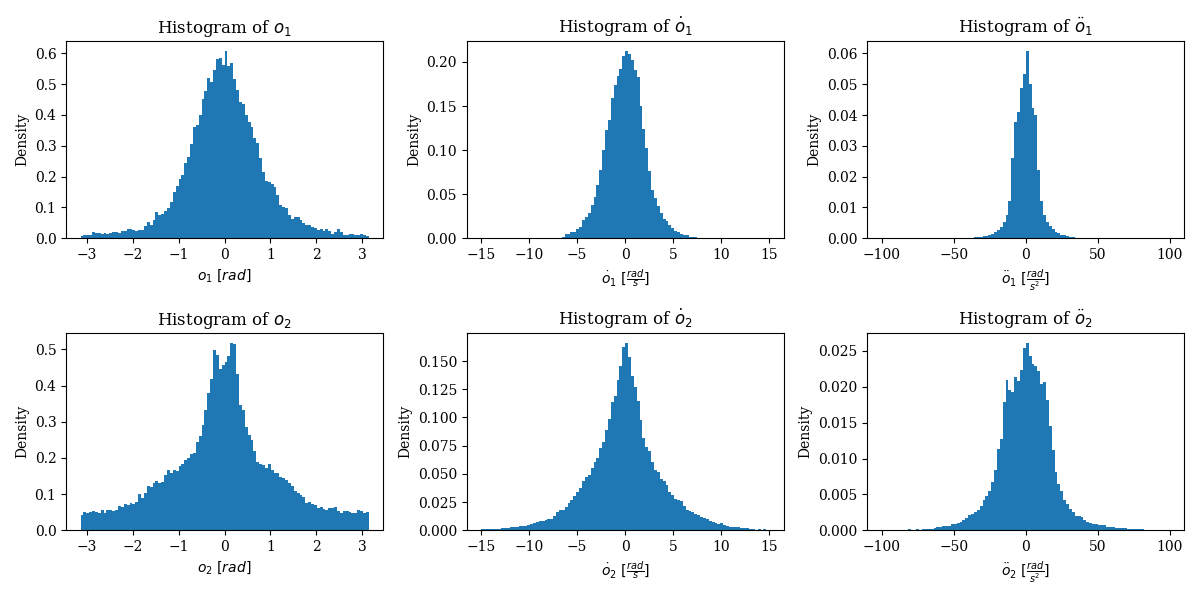
\includegraphics[width=\linewidth]{histogram_pendulum_lowfrict.png}
            \vspace{0.2em}
            \scriptsize \textcolor{orange}{Low Friction}
        \end{column}
        
    \end{columns}

    \vspace{0.5cm} 

    % --- LOWER ROW ---
    \centering
    \begin{minipage}{0.48\textwidth} 
        \centering
        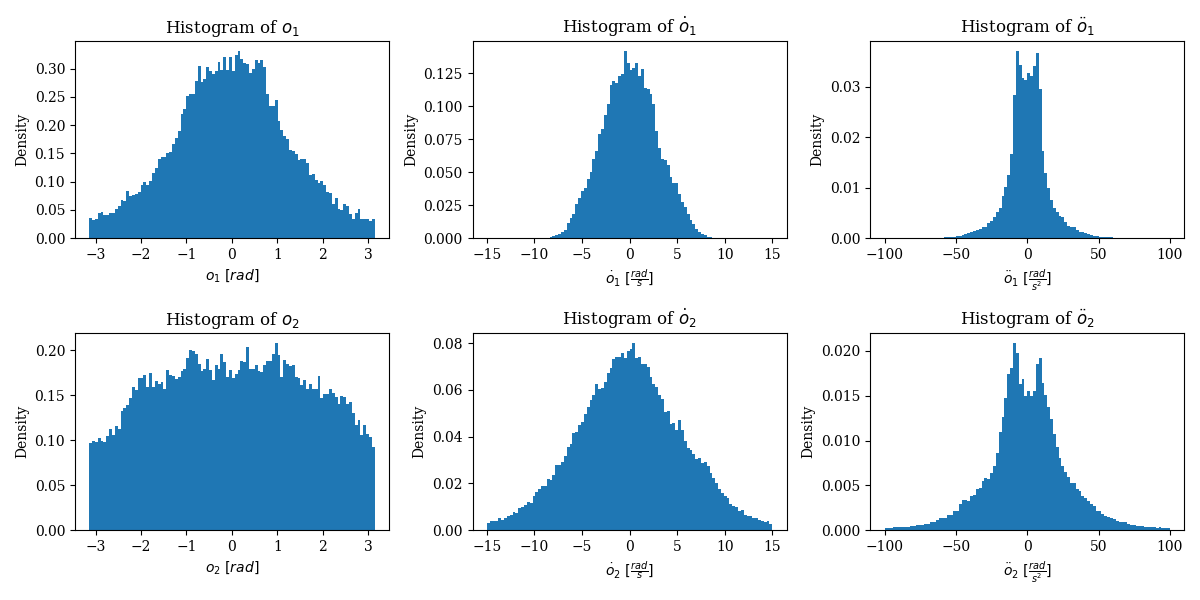
\includegraphics[width=\linewidth]{histogram_pendulum_nofrict.png}
        \vspace{0.2em}
        \scriptsize \textcolor{red}{No Friction}
    \end{minipage}

\end{frame}

%------------------------------------------------

\subsection{Preprocessing}

